\documentclass[12pt]{article}

\usepackage{fullpage}
\usepackage{graphicx, rotating, booktabs} 
\usepackage{times} 
\usepackage{natbib} 
\usepackage{indentfirst} 
\usepackage{setspace}
\usepackage{grffile} 
\usepackage{hyperref}
\usepackage{adjustbox}
\usepackage{amsmath}
\usepackage{siunitx}
\setcitestyle{aysep{}}


\singlespace
\title{\textbf{Appendix: Democracy, Elections, and Alliance Treaty Depth}}
\author{}
\date{}

\bibliographystyle{apsr}

\begin{document}

\maketitle 

\doublespace 

This appendix checks the findings in the manuscript in four ways. 
In the first section, I show results with several alternative model specifications and a bivariate model of depth and unconditional military support.
Then, I assess other ways of measuring treaty depth. 
After that, I consider some interesting findings of a negative correlation between military institutionalization and alliance performance. 
In the final section, I consider how uncertainty in the latent depth measure affects inferences about the association between democracy and treaty depth. 


\section{Alternative Model Specifications} 


In addition to robustness checks with alternative measures of electoral democracy, I fit two models with a crucial control. 
Perhaps the positive association between electoral democracy and treaty depth is driven by the United States, which formed multiple deep alliances after 1945. 
To assess this possibility, I add a dummy indicator of US membership to the beta model specification in the manuscript. 
\autoref{tab:us-reg} summarizes the resulting estimates. 
Even after adjusting for US membership, the same patterns hold- electoral democracy in the most capable alliance member increases treaty depth. 
 

\begin{table}[!htbp] \centering  
\begin{tabular}{@{\extracolsep{5pt}}lcc} 
\\[-1.8ex]\hline 
\hline \\[-1.8ex] 
 & \multicolumn{2}{c}{\textit{Dependent variable:}} \\ 
\cline{2-3} 
\\[-1.8ex] & \multicolumn{2}{c}{Latent Depth (rescaled)} \\ 
\\[-1.8ex] & (1) & (2)\\ 
\hline \\[-1.8ex] 
 Lexical Index of Democracy & 0.223$^{}$ & 0.264$^{}$ \\ 
  & (0.125, 0.320) & (0.133, 0.395) \\ 
  Executive Constraints & $-$0.885$^{}$ & $-$1.129$^{}$ \\ 
  & ($-$1.357, $-$0.412) & ($-$1.850, $-$0.409) \\ 
  Economic Issue Linkage & $-$0.209 & $-$0.353 \\ 
  & ($-$0.528, 0.109) & ($-$0.791, 0.085) \\ 
  Unconditional Support & 0.461$^{}$ & 0.588$^{}$ \\ 
  & (0.149, 0.774) & (0.188, 0.988) \\ 
  Foreign Policy Concessions & $-$0.060 & $-$0.170 \\ 
  & ($-$0.224, 0.105) & ($-$0.415, 0.075) \\ 
  Number of Members & 0.032$^{}$ & 0.063$^{}$ \\ 
  & (0.005, 0.059) & (0.024, 0.102) \\ 
  Wartime Alliance & $-$0.025 & $-$0.270 \\ 
  & ($-$0.401, 0.352) & ($-$1.276, 0.737) \\ 
  Asymmetric Obligations & 0.247 & 0.295 \\ 
  & ($-$0.098, 0.592) & ($-$0.307, 0.897) \\ 
  Asymmetric Capability & 0.312 & 0.535 \\ 
  & ($-$0.156, 0.780) & ($-$1.658, 2.727) \\ 
  Non-Major Only & 0.149 & 0.504 \\ 
  & ($-$0.365, 0.662) & ($-$1.708, 2.717) \\ 
  Average Threat & 1.033$^{}$ & 0.873 \\ 
  & (0.196, 1.870) & ($-$0.317, 2.063) \\ 
  Foreign Policy Disagreement & 0.245 & 0.071 \\ 
  & ($-$0.229, 0.720) & ($-$0.686, 0.828) \\ 
  Post 1945 & 0.135 &  \\ 
  & ($-$0.254, 0.524) &  \\ 
  US Membership & 0.328 & 0.457 \\ 
  & ($-$0.276, 0.932) & ($-$0.347, 1.261) \\ 
  Constant & $-$2.011$^{}$ & $-$2.043 \\ 
  & ($-$2.801, $-$1.221) & ($-$4.514, 0.427) \\ 
 \hline \\[-1.8ex] 
Observations & 276 & 158 \\ 
Log Likelihood & 63.738 & 36.309 \\ 
\hline 
\hline \\[-1.8ex] 
\textit{Note:}  & \multicolumn{2}{r}{95\% Confidence Intervals in Parentheses.} \\ 
\end{tabular} 
  \caption{Beta regression estimates of the association between alliance leader electoral democracy and alliance treaty depth, controlling for US membership. Model 1 includes all alliances from 1816 on, while Model 2 includes only alliances after 1945.} 
  \label{tab:us-reg}
\end{table} 


\subsection{Alternative Measures of Electoral Competition}


Other democracy measures emphasize the presence of open and competitive elections. 
As such, these measures should generate similar inferences about the connection between democratic institutions and alliance treaty design. 
In this section, I assess three such measures, including one that conceptualizes democratic influence in terms of the proportion of alliance members with high electoral democracy. 


The first measure of electoral competition is an dummy measure based on the Polity data's executive recruitment concept.  
When the most capable alliance member has competitive elections, I set this dummy variable to one, and zero otherwise. 
72 alliances have a leader with electoral competition, according to the Polity criteria. 


The other measure of electoral democracy builds off of the concept of polyarchy \citep{Dahl1971}, which includes both contestation and electoral inclusiveness. 
Polyarchy relies on both the opportunity and freedom of actors to compete in elections for leadership, as leaders must address voters' preferences to avoid being removed from office. 
It places more weight on inclusive participation in politics beyond elections than the lexical index of democracy, however. 
To measure polyarchy, I use the polyarchy measure of electoral democracy from the Varieties of Democracy dataset \citep{Teorelletal2016}.
As with the lexical index of democracy, I measure polyarchy in the most capable alliance member in the year the treaty formed.



As a further check, I translated my electoral democracy measure into an alternative conceptualization of democratic influence--- the proportion of democracies in the alliance.
\citet{Chibaetal2015} use the proportion of democracies as their key independent variable, and code this variable as the share of alliance members with a Polity score above 5 when the alliance formed. 
A greater proportion of electoral democracies should also increase alliance treaty depth, as democratic concerns have more weight, and the leading state is more likely to be democratic. 
I express the proportion of electoral democracies as the share of alliance members with a score of four or higher on the electoral index of democracy. 
I also control for the share of alliance members with executive constraints. 
Because democracies cooperate more with one another \citep{Leeds1999}, the proportion measures are positively correlated with the democratic institutions of the most capable alliance member. 
 
I then fit the same models of treaty depth and replaced the lexical index of electoral democracy with the three alternative measures.
All of these models retain the executive constraints variable from Polity, as this variable is correlated with electoral competition and alliance treaty design. 
In \autoref{fig:results-other-democ}, I plot the substantive impact of moving from the minimum to the maximum of the key independent variable. 
These substantive effect calculations hold all other variables in the model constant, and I fix executive constraints to one. 
Each figure in the plot contains three estimates--- the predicted outcome with the key independent variable at its minimum value, the same predictions with the variable at its maximum, and the difference between the two scenarios. 


\begin{figure}[hbtp]
\centering
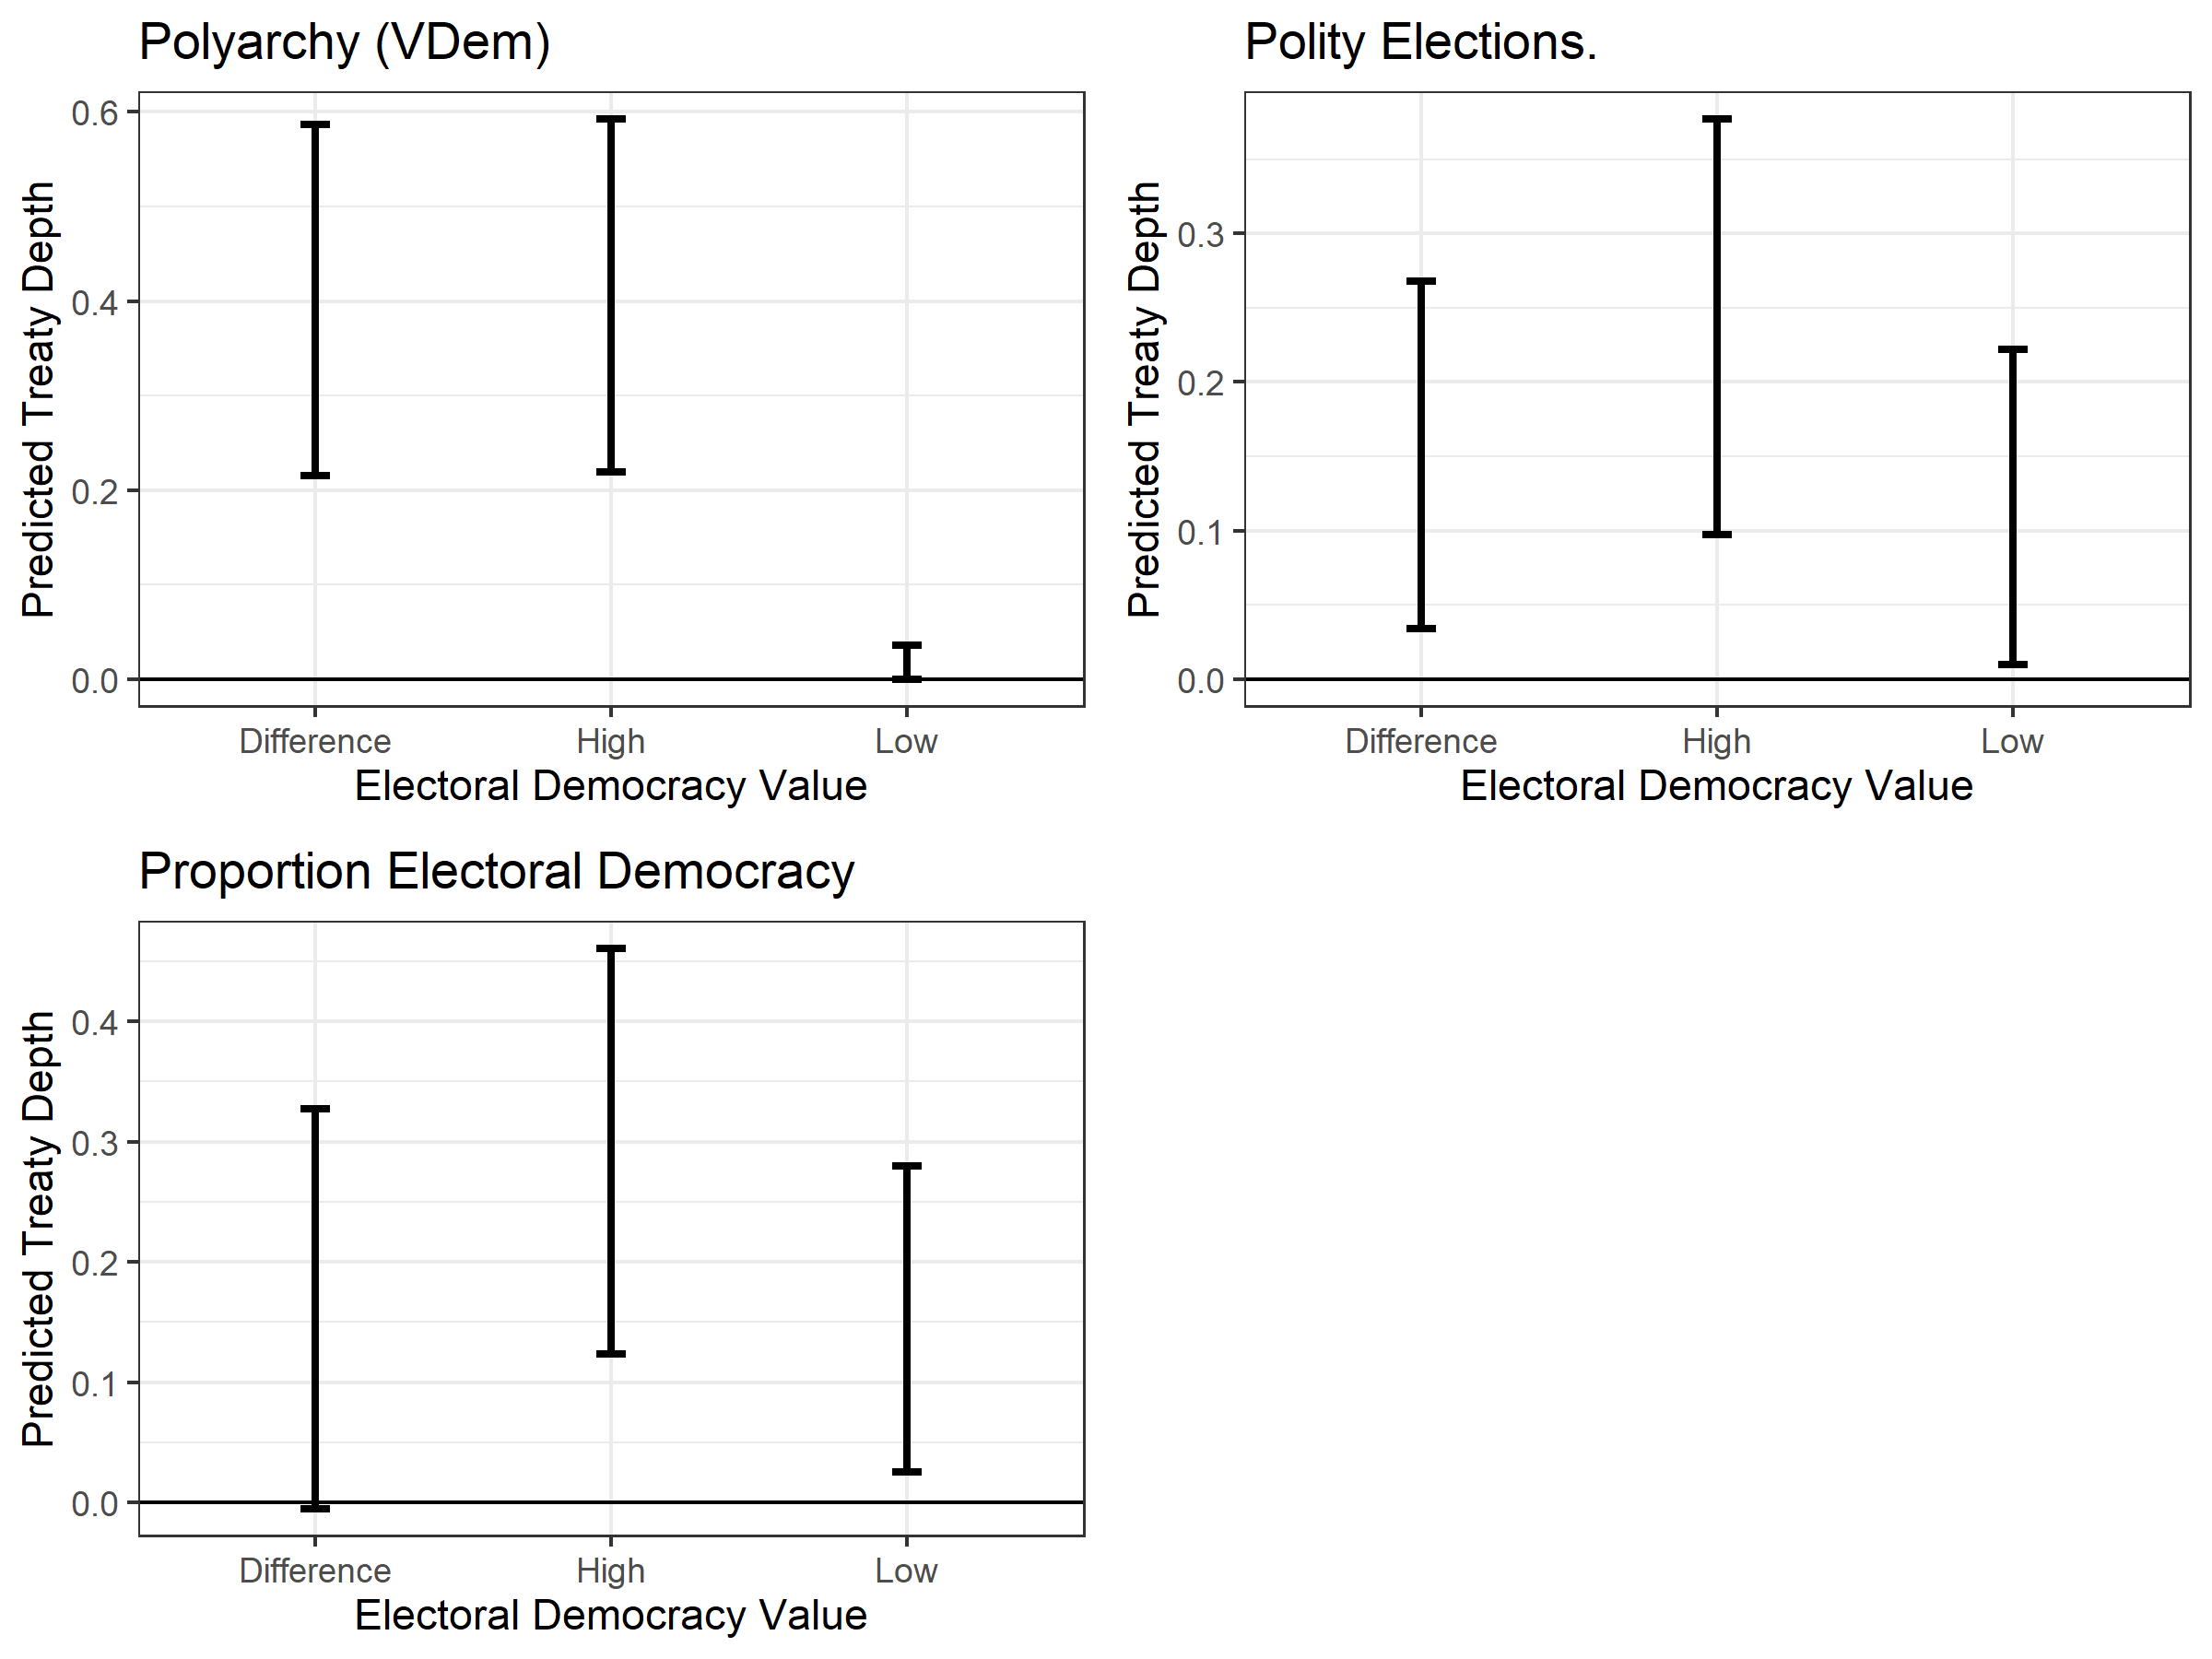
\includegraphics[width=0.95\textwidth]{results-other-democ.png}
\caption{Predicted treaty depth and probability of unconditional military support in offensive and defensive alliances from 1816 to 2007, all else equal besides an indicator of electoral competition. For each measure of electoral democracy, this figure shows the estimated treaty depth or probability of unconditional military support when electoral democracy is at maximum or minimum, along with the difference between the two scenarios.}
\label{fig:results-other-democ}
\end{figure}


Results with proportion of alliance members that have high electoral democracy partially match my hypotheses.  
The predicted difference in treaty depth between the low and high extent of electoral competition among alliance members is largely positive, but overlaps zero. 
Inferences about the association between the polity measure of electoral competition and alliance treaty design are also consistent with the argument that elections lead to greater alliance treaty depth.
Moving from no electoral competition to competition increases depth by between .03 and .27, which is a large effect relative to the range of rescaled treaty depth. 
As expected, greater electoral democracy as measured by the Varieties of Democracy polyarchy index increases treaty depth by between .21 and .59.
This large result reflects a move from a polyarchy score of 0 to a score of .9. 
In summary, these alternative measures give similar inferences about a positive association between alliance leader electoral democracy and treaty depth. 




\subsection{Bivariate Models of Depth and Unconditional Military Support}


I also use a bivariate statistical model to examine how democratic political institutions affect treaty depth.\footnote{Bivariate refers to a model means two outcome variables, not a model with one independent and one dependent variable.} 
Two factors encourage this research design choice. 
First, \citet{FjelstulReiter2019}, who note that different alliance treaty design decisions are correlated.
Because depth and conditions on support both build credibility, it is possible that they are related. 
Bivariate estimation also accounts for correlated errors because common unobserved factors may affect depth and conditionality \citep{Braumoelleretal2018}.
Independent univariate models assume that alliance treaty design decisions are uncorrelated, if this assumption is violated, biased estimates may result. 
My approach here is analogous to the well-known bivariate probit model, but it is not fully recursive, because I do not include depth or unconditional military support as endogenous predictors.\footnote{A fully recursive model requires two instruments for identification, and valid instruments are hard to find in alliance politics.}  
Instead, this model assumes that states make decisions about depth and conditions on military support at the same time. 


I use a generalized joint regression model (GJRM) \citep{Braumoelleretal2018} to combine the probit and beta specifications in a bivariate model.
This flexible estimator takes the probit and beta models and employs non-linear smoothed terms for threat and the start year of the alliance while estimating error term correlations. 
Adjusting for unobserved correlations between depth and unconditional military support ensures accurate inferences about democracy and other covariates.
GJRM uses copulas to model correlated errors in multiple equation models, which makes it more flexible than parametric models and facilitates causal inference. 
Copulas are distributions over functions, and they relax potentially problematic assumptions about the shape of the correlation in the error terms. 
Because controlling for error term correlations is crucial for inferences about correlated data-generating processes, considering a flexible set of functions to capture the error distributions ensures that the results are not an artifact of parametric assumptions. 
I fit models with every possible copula, and selected the best-fitting model using AIC, conditional on that estimator having converged.\footnote{GJRM uses maximum likelihood estimation, and diagnostics for the gradient as well as the information matrix suggest that the models behind all inferences in the paper and appendix converged.} 
The student-t copula maximizes model fit. 


A third equation in the GJRM estimator models heterogeneity in the error term correlations, which is important because depth and unconditional support could be positively correlated in some alliances, and negatively correlated in others. 
Correlations in unobservable factors between treaty depth and unconditional promises of military spending could also vary with the international context.
For example, \citet{Kuo2019} shows how European politics encouraged the proliferation of secret alliances before World War I, and similar processes of emulation and diffusion may operate over time.
Last, multilateral alliances are likely to encourage deep and conditional obligations, as members hedge against entrapment and coordinate through treaty depth. 
I use the start year of the alliance, the number of members and democratic institutions to predict the error term correlations.
To address the start year of the alliance, I include a smoothed term for the start year of the alliance in the error term equation.  


In summary, the GJRM model is a general and flexible way to simultaneously model different aspects of alliance treaty design.
Like the measurement model, it uses a semiparametric approach to relax potentially problematic assumptions about the distribution of underlying correlations. 
It also allows me to model the two outcomes with appropriate distributions. 
\autoref{tab:gjrm-res} shows the estimates from this model specification. 
I find the same results with a binary measure of electoral democracy- high electoral democracy increases treaty depth.
I also find that electoral democracy decreases the probability of unconditional military support. 


\begin{table}[ht]
\centering
\begin{tabular}{lrrrr}
  & \multicolumn{2}{c}{Uncond. Mil. Support} & \multicolumn{2}{c}{Latent Depth}\\ \hline
  & Estimate & Std. Error & Estimate & Std. Error \\ 
  \hline
  Executive Constraints & 0.9060546 & 0.3047151 & -0.4145406 & 0.1997270 \\ 
  Lexical Index of Democracy & -0.1912880 & 0.0593793 & 0.1311648 & 0.0428888 \\ 
  Economic Issue Linkage & 0.0856345 & 0.1622075 & 0.0089622 & 0.1276000 \\ 
  FP Concessions & 0.0034752 & 0.0943471 & -0.0710498 & 0.0714206 \\ 
  Number of Members & -0.1427829 & 0.0249413 & 0.0339447 & 0.0141152 \\ 
  Wartime Alliances & -0.7083312 & 0.2291947 & -0.0909938 & 0.1697764 \\ 
  Asymmetric Obligations & -0.1716237 & 0.2388670 & 0.2774828 & 0.1627990 \\ 
  Asymmetric Capability & 1.5636757 & 0.4878849 & 0.5100054 & 0.2279664 \\ 
  Non-Major Only & 2.3127385 & 0.4694387 & 0.1804889 & 0.2286315 \\ 
  FP Disagreement & 0.4956369 & 0.2497704 & 0.3324241 & 0.1876389 \\ 
  s(Mean Threat) & 7.7375312 & 93.3416610 & 1.0000001 & 22.4454954 \\ 
  s(Start Year) & 6.4470418 & 132.2791467 & 4.1045361 & 30.4155941 \\ 
  (Intercept) & -1.5231481 & 0.5081536 & -1.4846432 & 0.2753943 \\ 
   \hline
\end{tabular}
\caption{Results from a joint generalized regression model of treaty depth and unconditional military support in 
         offensive and defensive alliances from 1816 to 2007. 
                     All smoothed terms report the effective degrees of freedom and the chi-squared term. 
                     The unconditional military support model is a binomial GLM with a probit link function. 
                     The treaty depth model is a beta regression. 
                     I model the error correlation between the two processes with a T copula.} 
\label{tab:gjrm-res}
\end{table}





\section{Other Measures of Treaty Depth}



Besides estimating the association between democracy and depth without rescaling the outcome, I examine the relationship between alliance leader democracy and two measures from earlier scholarship that capture parts of treaty depth. 
First, \citet{LeedsAnac2005} develop an ordinal measure of military institutionalization.
Second, \citet{BensonClinton2016} use a latent variable model to measure treaty depth, but they conceptualize depth as the overall costliness of the alliance obligations. 
Although these two measures have limitations that make my measure a better fit for this paper, I find that the electoral democracy of the alliance leader is positively correlated with both variables.


Greater alliance leader electoral democracy increases the Leeds and Anac measure of military institutionalization in separate and joint models.
The ordinal military institutionalization measure is a useful first step towards measuring defense cooperation, but it understates the amount of variation in treaty depth. 
\citet{LeedsAnac2005} argue that commitments of an integrated military command, common defense policy, or any basing rights generate high military institutionalization. 
Official contact between military officials, formal organizations, providing training or technology, subordination of forces, or specific contributions reflect moderate institutionalization. 
If at least one of the relevant factors is present, Leeds and Anac assign the alliance the highest corresponding level of institutionalization. 
To give an example, an alliance with basing rights and subordination of forces has high institutionalization and is just as institutionalized as an alliance with only basing rights. 
This approach assumes that alliances with multiple sources of depth as just as deep or institutionalized as alliances with one source.
As a result, it understates variation in alliance treaty depth.


\begin{figure}[htbp]
	\centering
		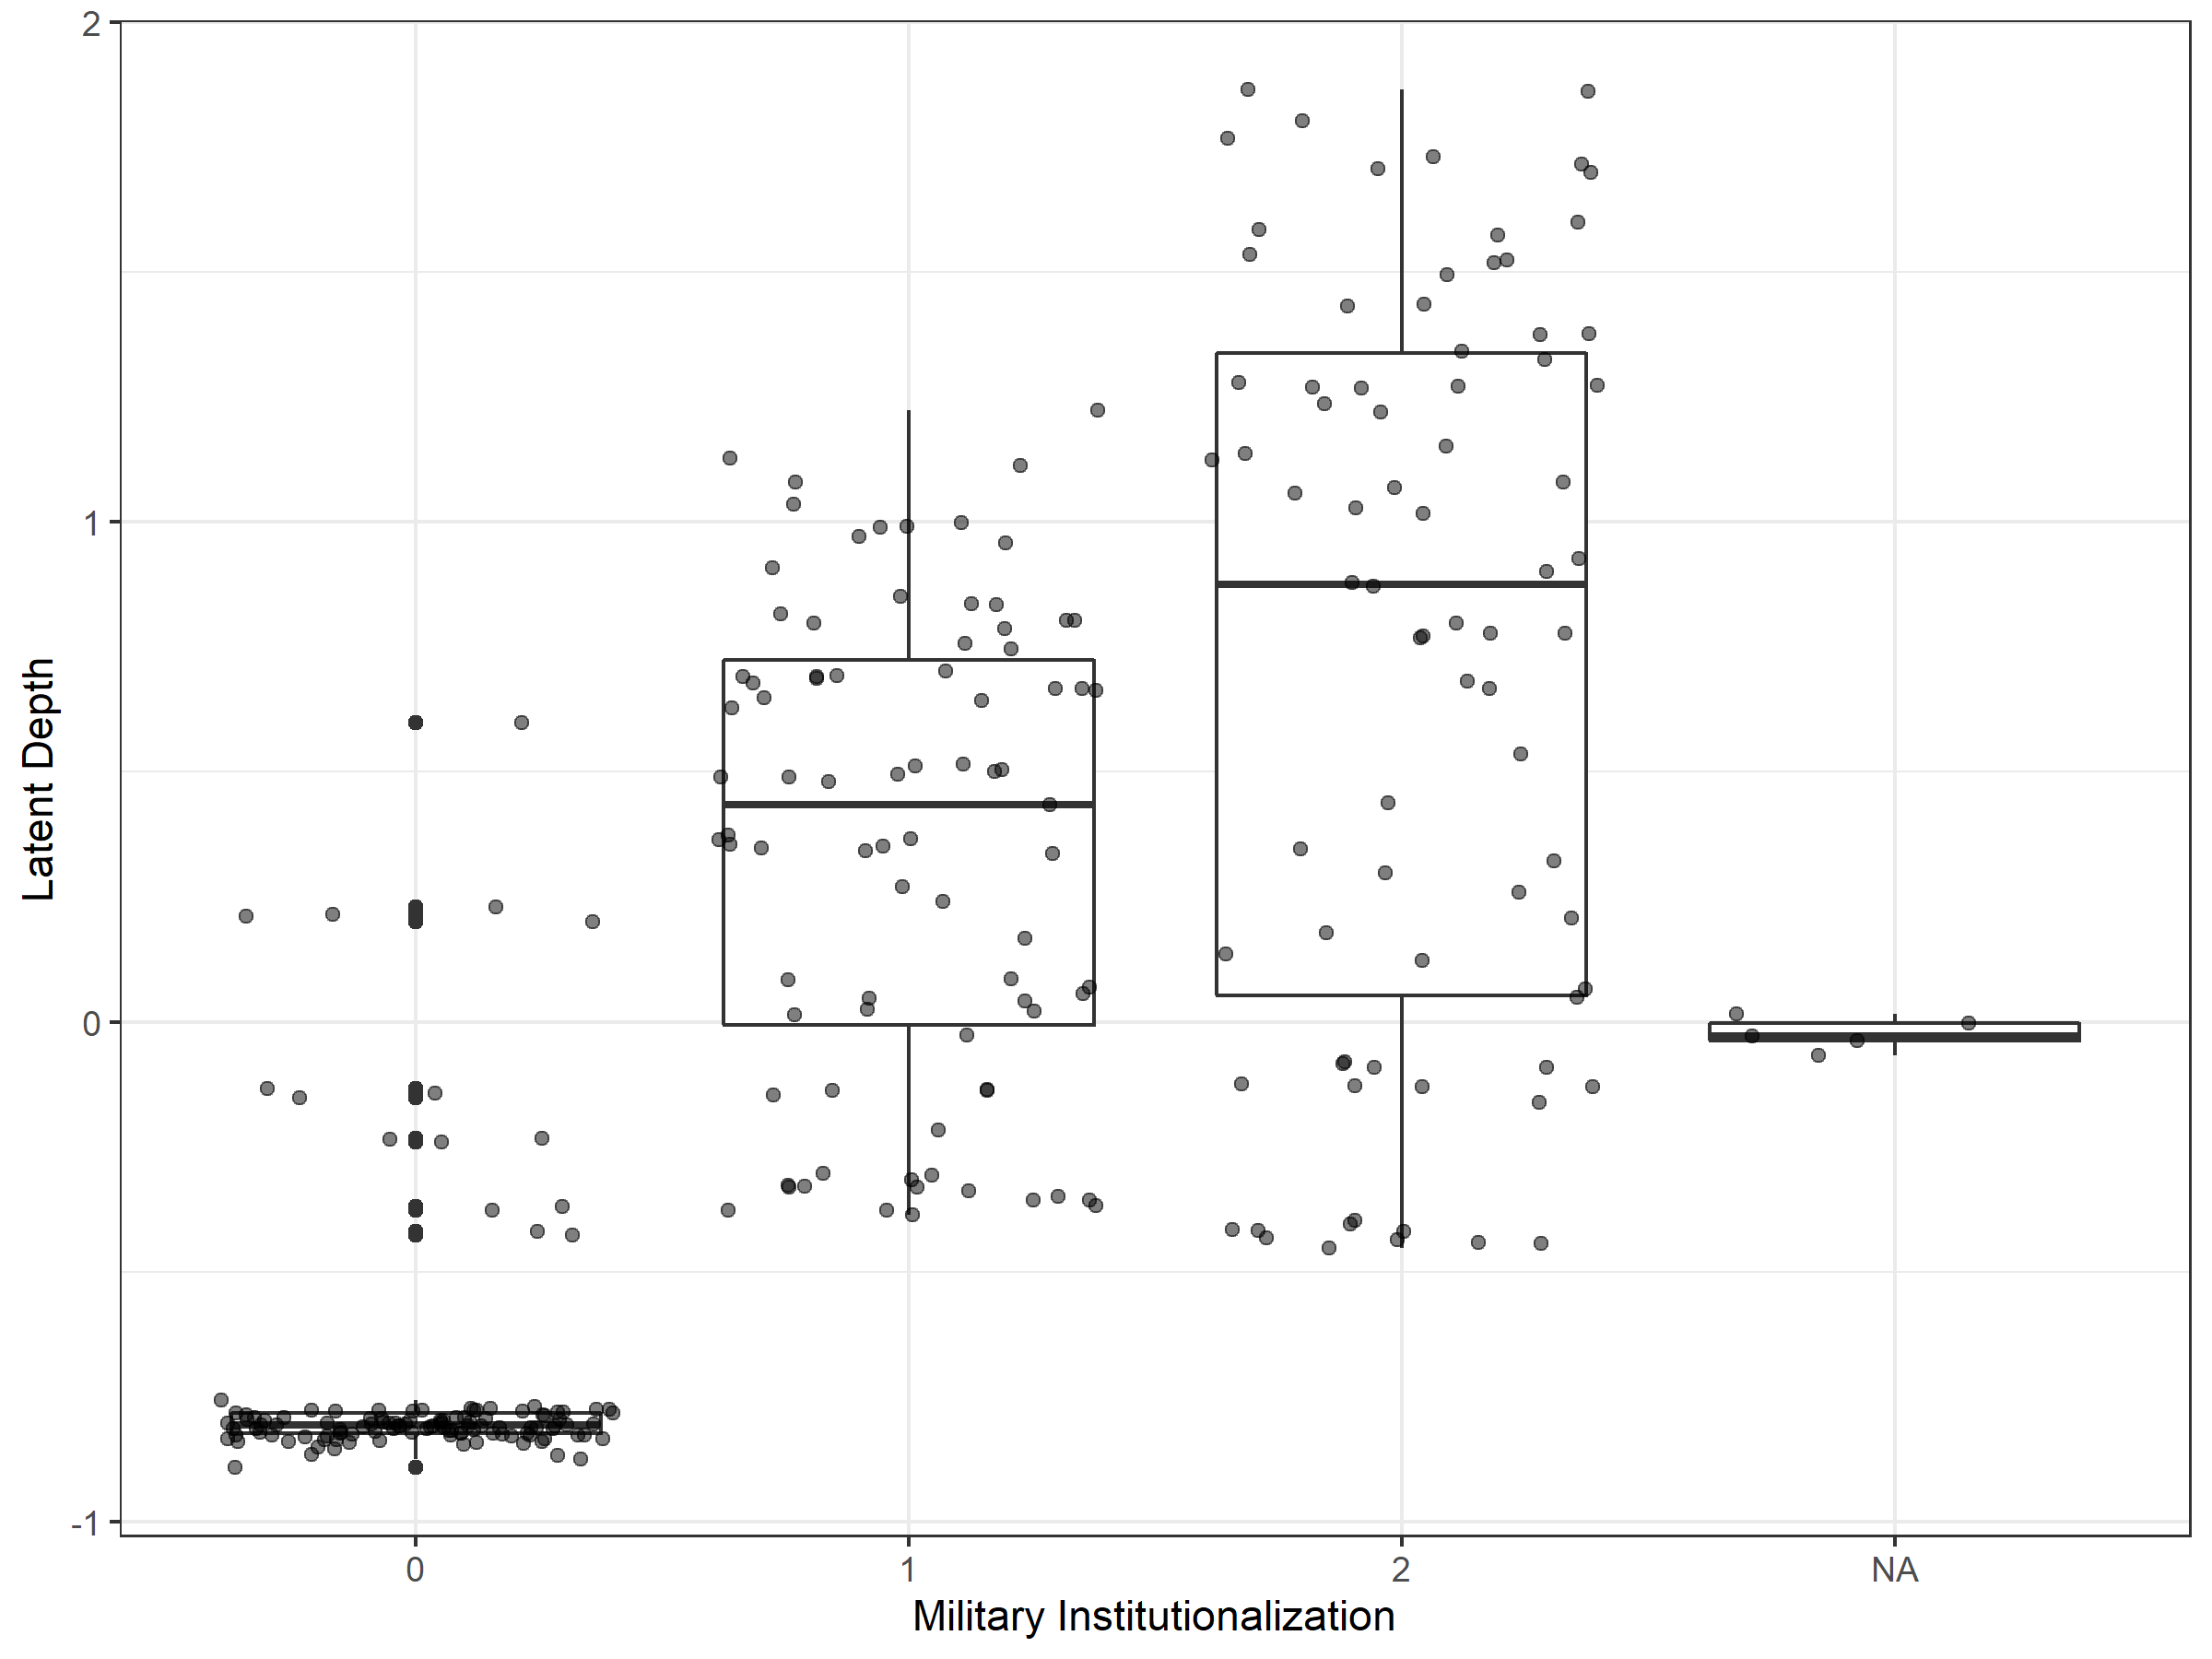
\includegraphics[width=0.95\textwidth]{milinst-comp.png}
	\caption{Scatter plot of latent treaty depth across the values of military institutionalization from \citet{LeedsAnac2005}. The box plots summarize the distribution of latent treaty depth within each category of military institutionalization. Points are jittered within each level of the institutionalization score.}
	\label{fig:milinst-comp}
\end{figure} 


As \autoref{fig:milinst-comp} shows, the ordinal variable is positively correlated with my latent measure, but the latent depth measure varies widely within each level. 
The deepest alliances on the latent measure also have the highest military institutionalization score.
There are substantial differences within each category and overlap in the latent scores across the categories, however. 
For example, some alliances that \citet{LeedsAnac2005} assign a moderate institutionalization score have more depth than alliances with high institutionalization scores because these alliance treaties contain multiple sources of depth. 


\citet{BensonClinton2016}'s measure addresses a different concept, covers fewer alliances and their measurement model relies on a set of potentially problematic distributional assumptions, so it produces more outliers that may impact inferences.
Benson and Clinton's emphasis on the general costliness of the alliance means they include measures of issue linkages and secrecy, which are distinct from defense cooperation. 
Their measure is also based on version 3 of the ATOP data, so it has more limited temporal coverage. 
Last, their latent variable model makes a series of distributional assumptions that affect the estimated distribution of the latent depth measure. 
My latent variable model uses a semiparametric approach that accounts for dependencies between the factors and latent variables, so the distribution of the latent variable may be more accurate \citep{Murrayetal2013}.
For these three reasons, my latent measure better captures the concept of defense coordination and cooperation.\footnote{If scholars want to measure the overall costliness of alliance obligations, they should consider Benson and Clinton's measure.} 
Despite these differences, I find a positive association between the lexical index of democracy in the most capable alliance member and Benson and Clinton's measure of depth. 


I now discuss the results of analyses with both alternative dependent variables. 
First, I fit an ordinal model of military institutionalization. 
Then, after rescaling Benson and Clinton's depth measure to range between 0 and 1, I fit a beta regression model. 
\autoref{fig:results-alt-measures-sep} plots the substantive effect of the most capable alliance member's lexical index of electoral democracy score on both outcomes. 
Electoral democracy in the alliance leader increase the probability of high institutionalization and decrease the probability of no institutionalization. 
Alliance leader democracy is also positively associated with Benson and Clinton's measure of depth. 


\begin{figure}
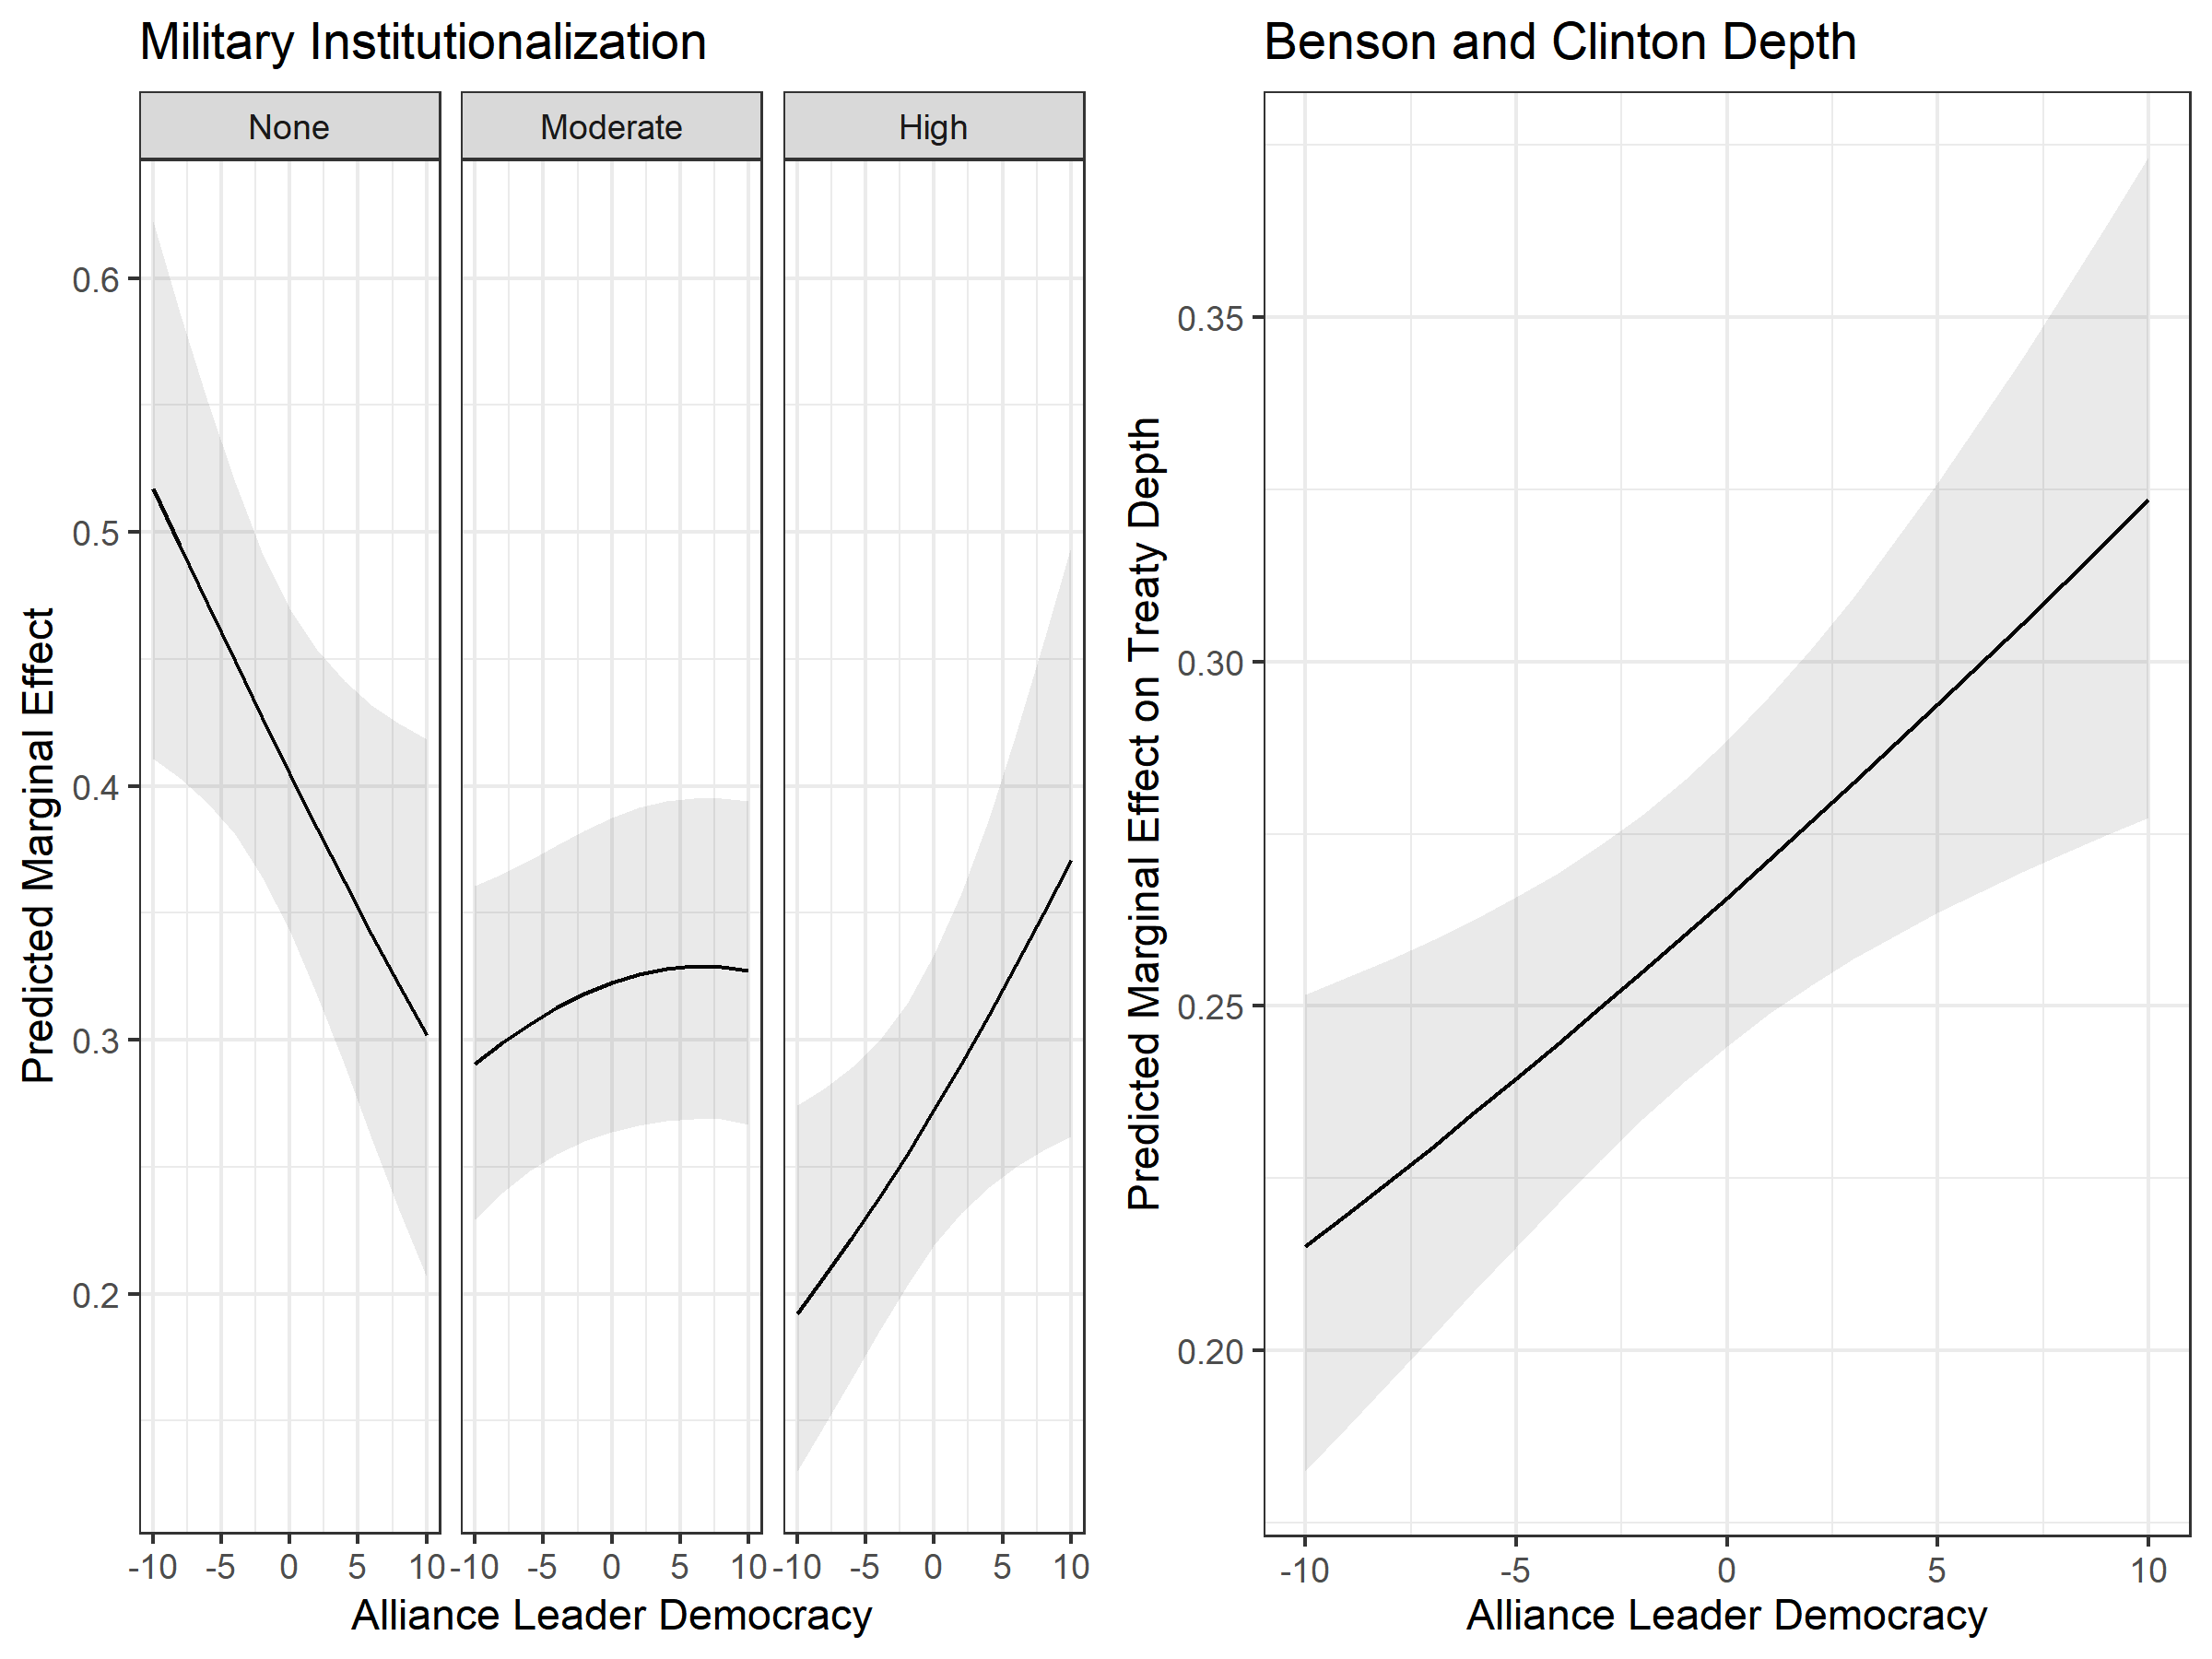
\includegraphics[width=.95\textwidth]{results-alt-measures-sep.png}  
\caption{Predicted changes in treaty depth by the electoral democracy of the most capable alliance member. The line marks predicted values, and the shaded areas encapsulate the 95\% confidence interval.}
\label{fig:results-alt-measures-sep}
\end{figure}



\subsection{Skew-T and Skew-Cauchy Models}

To address a highly skewed distribution and facilitate inferences across a wide range of estimation strategies, results in the paper are based on rescaled mean latent treaty depth, which ranges between 0 and 1. 
I modeled the rescaled outcome with a beta distribution. 
I make similar inferences about treaty depth and the electoral democracy of the most capable alliance member when I estimate regression models of treaty depth without this transformation, however. 


Latent mean treaty depth is extremely skewed. 
This in turn leads to assumption violations and poor model fit with ordinary least squares estimators. 
To address this problem, I fit skew-t and skew-cauchy models of treaty depth.
Both these estimators model the skewed errors, and the skew-cauchy model allows for larger outliers.   
The skewed regressions accommodate non-normal residuals and influential observations that might bias inferences with OLS. 
I summarize the estimates from the skew models in \autoref{fig:skew-model-res}. 


\begin{figure}[htbp]
	\centering
		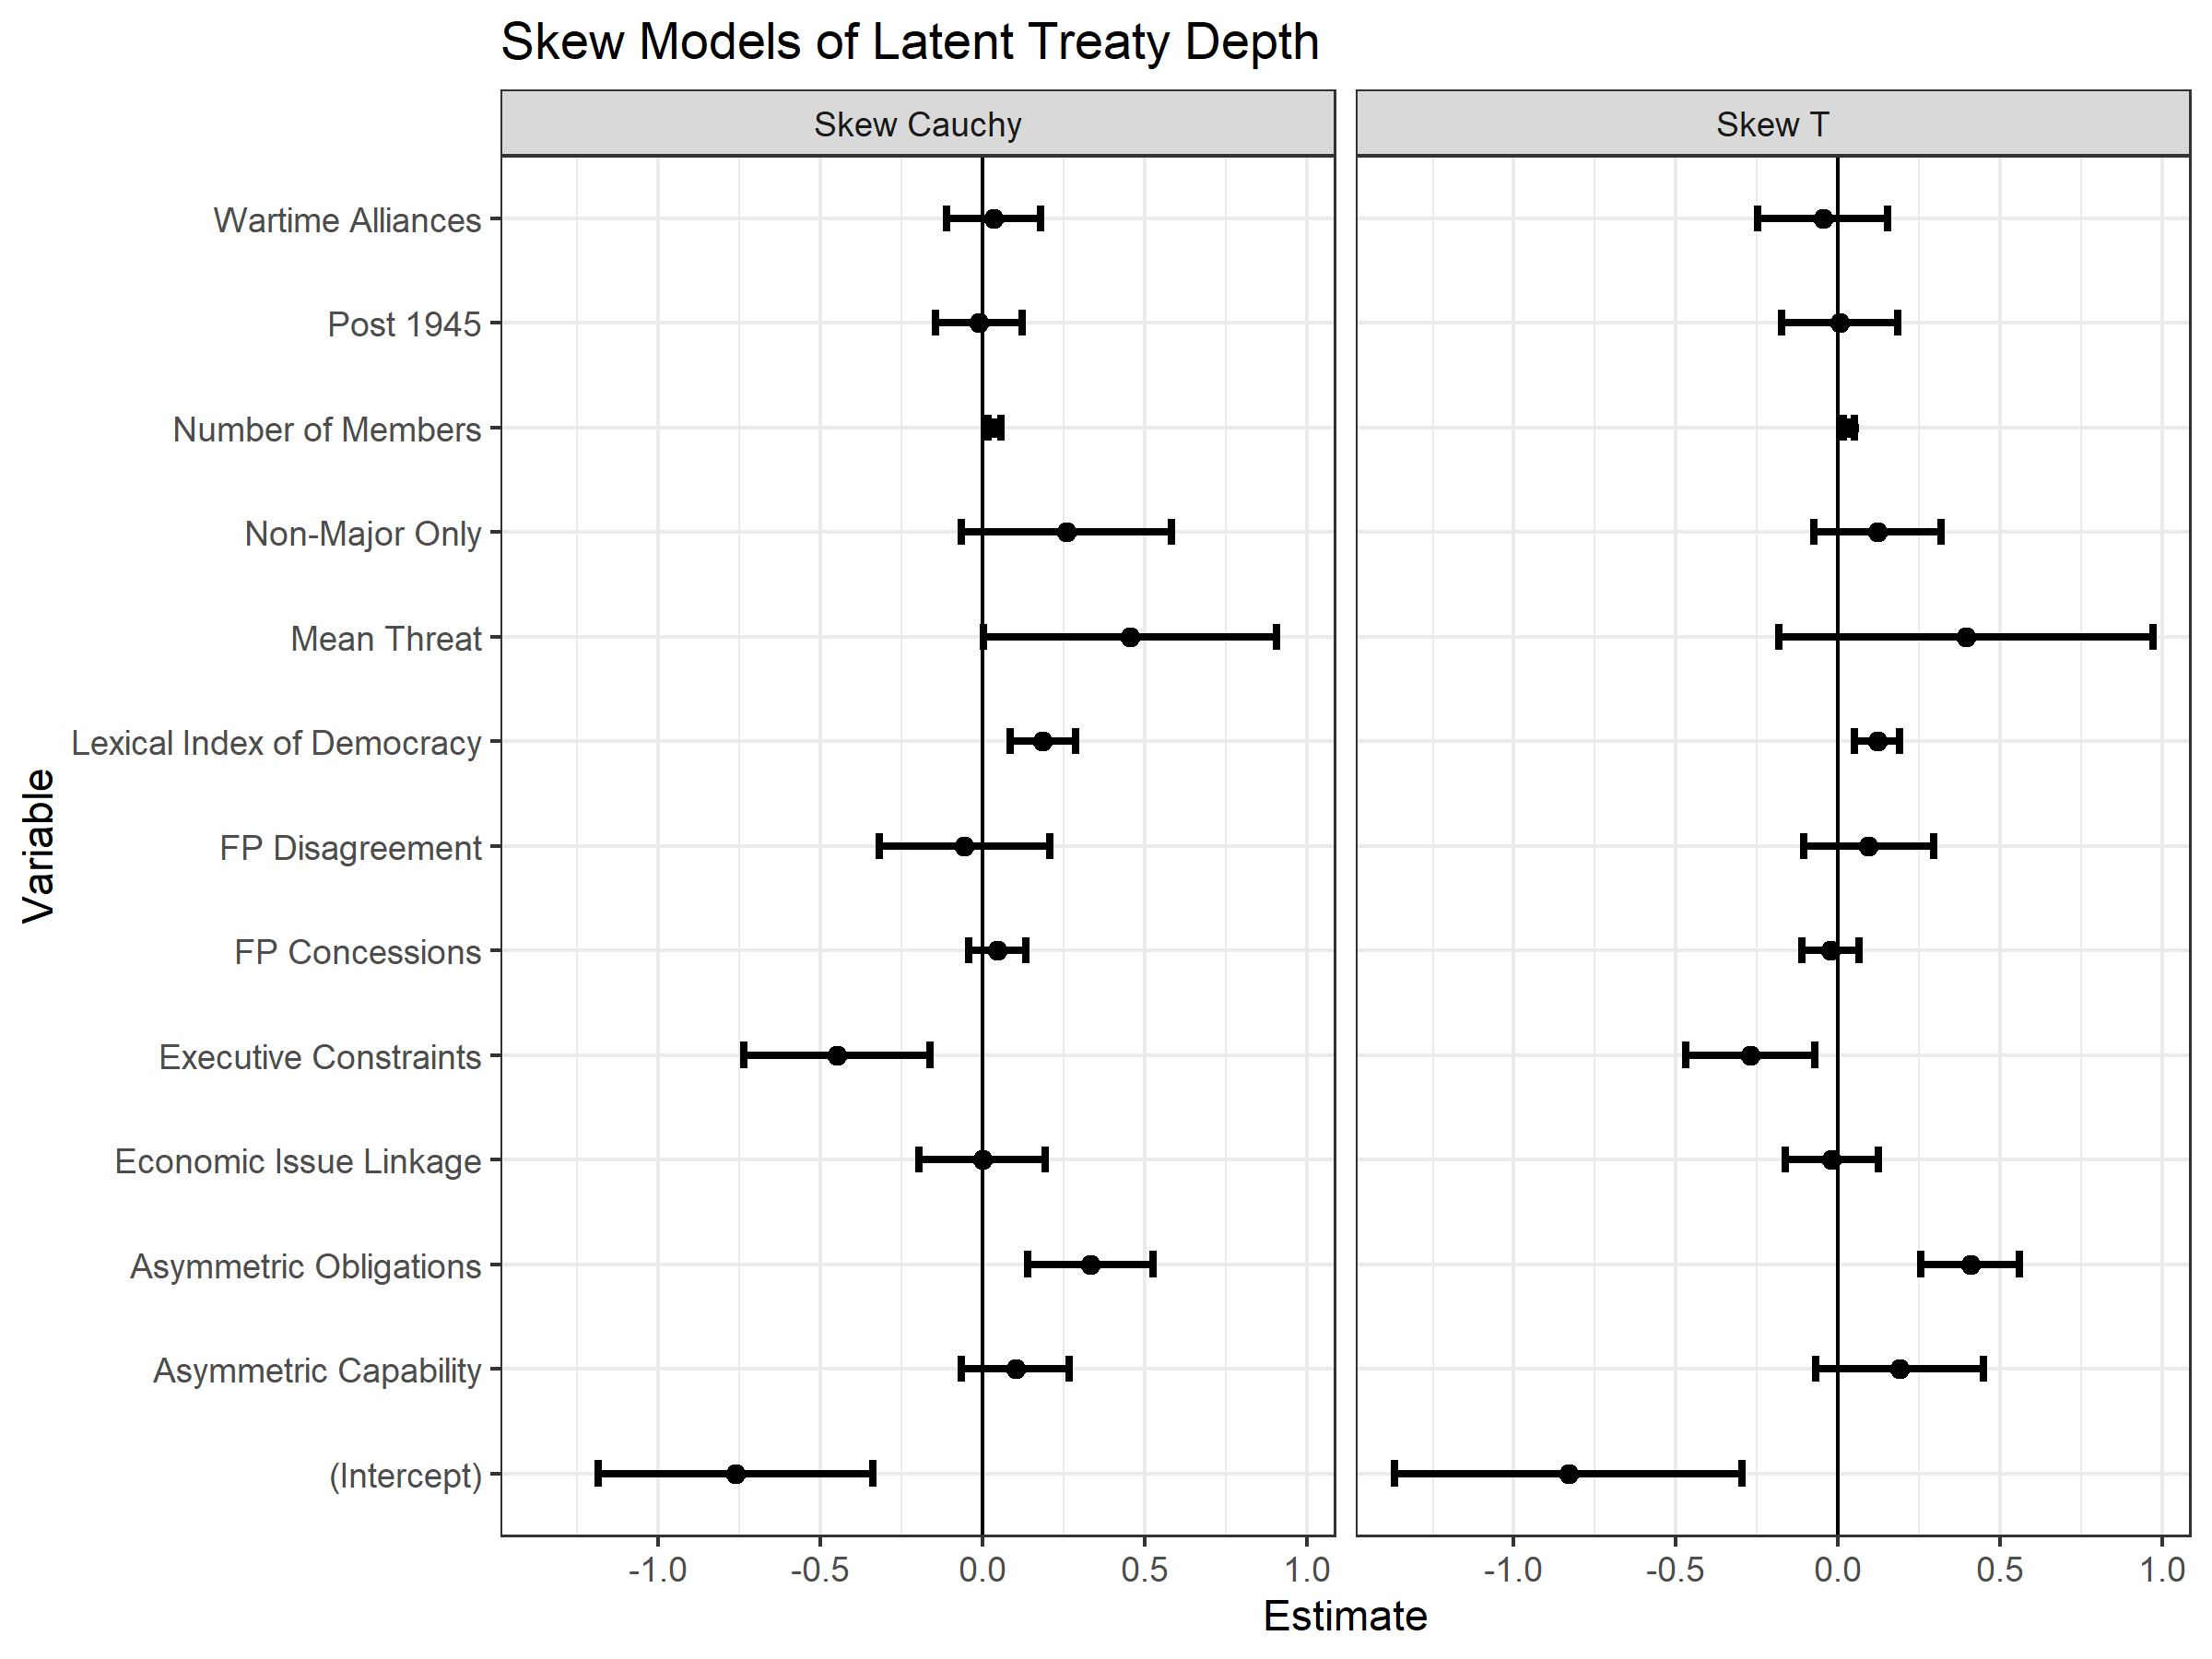
\includegraphics[width=0.95\textwidth]{skew-model-res.png}
	\caption{Coefficient plot of estimates from skew-t and skew-cauchy models of alliance treaty depth in offensive and defensive ATOP alliances from 1816 to 2012. Both estimators find a positive association between electoral democracy and treaty depth.}
	\label{fig:skew-model-res}
\end{figure} 


Without rescaling treaty depth, I still find a positive relationship between electoral democracy and alliance treaty depth. 
This inference also does not depend on how extreme the assumed skewness in the error terms is--- both the skew-t and skew-Cauchy estimators give similar inferences.  





\section{Are Deep Alliances Less Reliable?} 


\citet{LeedsAnac2005} find that alliance members are less likely to honor institutionalized alliances when members invoke the treaty.
These interesting findings contradict my claim that deep alliances increase treaty reliability, but may not reflect lackluster credibility of deep alliances. 
As \citet[pg. 198]{LeedsAnac2005} note, their results could be a function of non-random selection in alliance challenges \citep{Smith1995}. 
Furthermore, how treaty depth is measured affects inferences with Leed's and Anac's research design.
Replacing the ordinal measure with my continuous latent depth variable leads to different inferences about alliance treaty design and performance. 



I focus my replication on Leeds and Anac's model of whether alliance members honor treaties with active military support. 
The replication focuses on this model because my argument examines defensive and offensive alliances. 
Their dataset includes 103 alliance performance opportunities, where states could honor or violate promises of military support. 
Using a logit model that adjusts for alliance formality, capability changes, changes in the policy process and whether the ally was the original target, Leeds and Anac find a negative relationship between institutionalization and performance. 
I replicate this estimate in the first column of \autoref{tab:depth-performance}. 


\begin{table}[!htbp] \centering 
  \caption{} 
  \label{tab:depth-performance} 
\begin{adjustbox}{width= .95\textwidth, center}
\begin{tabular}{@{\extracolsep{5pt}}lccc} 
\\[-1.8ex]\hline 
\hline \\[-1.8ex] 
 & \multicolumn{3}{c}{\textit{Dependent variable:}} \\ 
\cline{2-4} 
\\[-1.8ex] & \multicolumn{2}{c}{Leeds and Anac} & Berkemeier and Fuhrmann \\ 
\\[-1.8ex] & (1) & (2) & (3)\\ 
\hline \\[-1.8ex] 
 Military Institutionalization & $-$0.543 &  &  \\ 
  & ($-$1.306, 0.221) &  &  \\ 
  Latent Depth &  & 0.258 & 0.347 \\ 
  &  & ($-$0.484, 1.000) & ($-$0.372, 1.066) \\ 
  Alliance Formality & $-$1.161$^{}$ & $-$1.538$^{}$ &  \\ 
  & ($-$2.082, $-$0.240) & ($-$2.483, $-$0.594) &  \\ 
  Capability Change & $-$1.841$^{}$ & $-$1.946$^{}$ &  \\ 
  & ($-$3.135, $-$0.547) & ($-$3.277, $-$0.614) &  \\ 
  Process Change & $-$1.802$^{}$ & $-$1.459$^{}$ &  \\ 
  & ($-$3.336, $-$0.269) & ($-$2.886, $-$0.032) &  \\ 
  Original Target & $-$0.723 & $-$0.836 &  \\ 
  & ($-$1.849, 0.403) & ($-$2.001, 0.329) &  \\ 
  Asymmetric Capability &  &  & $-$2.536$^{}$ \\ 
  &  &  & ($-$4.904, $-$0.168) \\ 
  Non-Major Only &  &  & $-$1.740 \\ 
  &  &  & ($-$3.954, 0.473) \\ 
  Post 1945 &  &  & $-$2.315$^{}$ \\ 
  &  &  & ($-$3.766, $-$0.864) \\ 
  Share Electoral Democracy &  &  & $-$0.217 \\ 
  &  &  & ($-$0.505, 0.070) \\ 
  Share Executive Constraints &  &  & $-$0.450 \\ 
  &  &  & ($-$1.587, 0.687) \\ 
  Number of Members &  &  & 1.054 \\ 
  &  &  & ($-$0.544, 2.653) \\ 
  Economic Issue Linkage &  &  & $-$0.093 \\ 
  &  &  & ($-$0.786, 0.600) \\ 
  Unconditional Support &  &  & 0.263 \\ 
  &  &  & ($-$2.343, 2.868) \\ 
  Foreign Policy Concessions &  &  & 1.799 \\ 
  &  &  & ($-$0.391, 3.989) \\ 
  Constant & 3.430$^{}$ & 3.201$^{}$ & 2.524$^{}$ \\ 
  & (1.972, 4.888) & (1.799, 4.602) & (0.182, 4.866) \\ 
 \hline \\[-1.8ex] 
Observations & 93 & 93 & 108 \\ 
Log Likelihood & $-$39.131 & $-$39.906 & $-$48.298 \\ 
\hline 
\hline \\[-1.8ex] 
\textit{Note:}  & \multicolumn{3}{r}{95\% Confidence Intervals in Parentheses.} \\ 
\end{tabular}
\end{adjustbox} 
\end{table}


I then replace Leeds and Anac's institutionalization measure with my latent treaty depth measure, which is in the second column of \autoref{tab:depth-performance}. 
The coefficient on depth, in contrast to military institutionalization, is positive, though neither estimate is statistically significant at conventional levels. 
Thus, the possible direction of this association shifts, depending on how alliance depth is measured.


To further assess this finding, I utilized an updated alliance performance dataset from \citet{BerkemeierFuhrmann2018}.
In this analysis, I specified a logit model that uses latent depth, unconditional support, dummy indicators of asymmetric capability and symmetric non-major power pacts, a post 1945 dummy, the two indicators of democratic membership, the number of members, economic issue linkages, and foreign policy concessions to predict whether an alliance was honored in war. 
All of these factors are potential sources of reliability and correlates of depth. 
In these models, I find a similar result--- a positive relationship between depth and honoring military support that cannot be distinguished from zero.


In summary, I do not find that highly institutionalized alliances are less reliable. 
The change in the direction of the coefficient is suggestive, given the limited number of alliance performance opportunities in these datasets. 
Again, given non-random selection into alliance crises and challenges, placing excessive weight on the above results is unwise. 
They do suggest, however, that deep alliances are not necessarily less reliable when invoked. 



\section{Uncertainty in Latent Treaty Depth} 


In a further robustness check, I consider how measurement uncertainty shapes inferences about the connection between electoral democracy and treaty depth. 
Although there are perceptible differences in treaty depth, especially once states add substantial depth to the treaty, the latent measure of treaty depth varies, as the model produces a distribution of plausible depth values for each alliances. 
This uncertainty in the latent measure is common to all measurement models and offers a reasonable approximation of alliance politics, because the implications of alliance treaty design are uncertain.  


To incorporate uncertainty over treaty depth, I fit a modification of the joint model. 
First, I created 1,000 alliance datasets, one for each draw of the posterior distribution of the latent measure.
All other variables remained the same, but the treaty depth values are unique to each dataset. 
Then I fit the treaty depth model on 400 randomly sampled datasets from those 1,000 using Bayesian estimation through BRMS \citep{Buerkner2017}. 
Joint Bayesian estimation has the flexibility to incorporate the probit and beta models and can be easily extended to account for uncertainty in the depth measure, but it does not allow correlated errors. 
Fitting the model sequentially to each dataset produces 400 separate models, which I combine into a single model by aggregating the posterior draws into a unified posterior that accounts for uncertainty in the treaty depth measure.\footnote{Standard convergence diagnostics indicate convergence in all 500 models. Diagnostics like $\hat{r}$ are less useful for the full posterior, because some of the chains in the submodels do not overlap.}
This approach is analogous to common techniques for analyzing missing data, where multiple imputation generates uncertainty about the missing values \citep{Hollenbachetal2018imp}.
After multiple imputation, researchers fit a separate model to each imputed dataset and then combine the results. 


% Expand on these results later 
Even after accounting for uncertainty in the treaty depth measure, I find a similar pattern. 
I plot the relevant posterior distributions in \autoref{fig:results-unc-depth}. 
The 95\% credible interval of the association between electoral democracy and depth is uniformly positive and 99\% of the posterior mass is positive. 
For executive constraints, the 95\% credible interval suggests a negative association, although these estimates do not account for selection into alliances. 


\begin{figure}
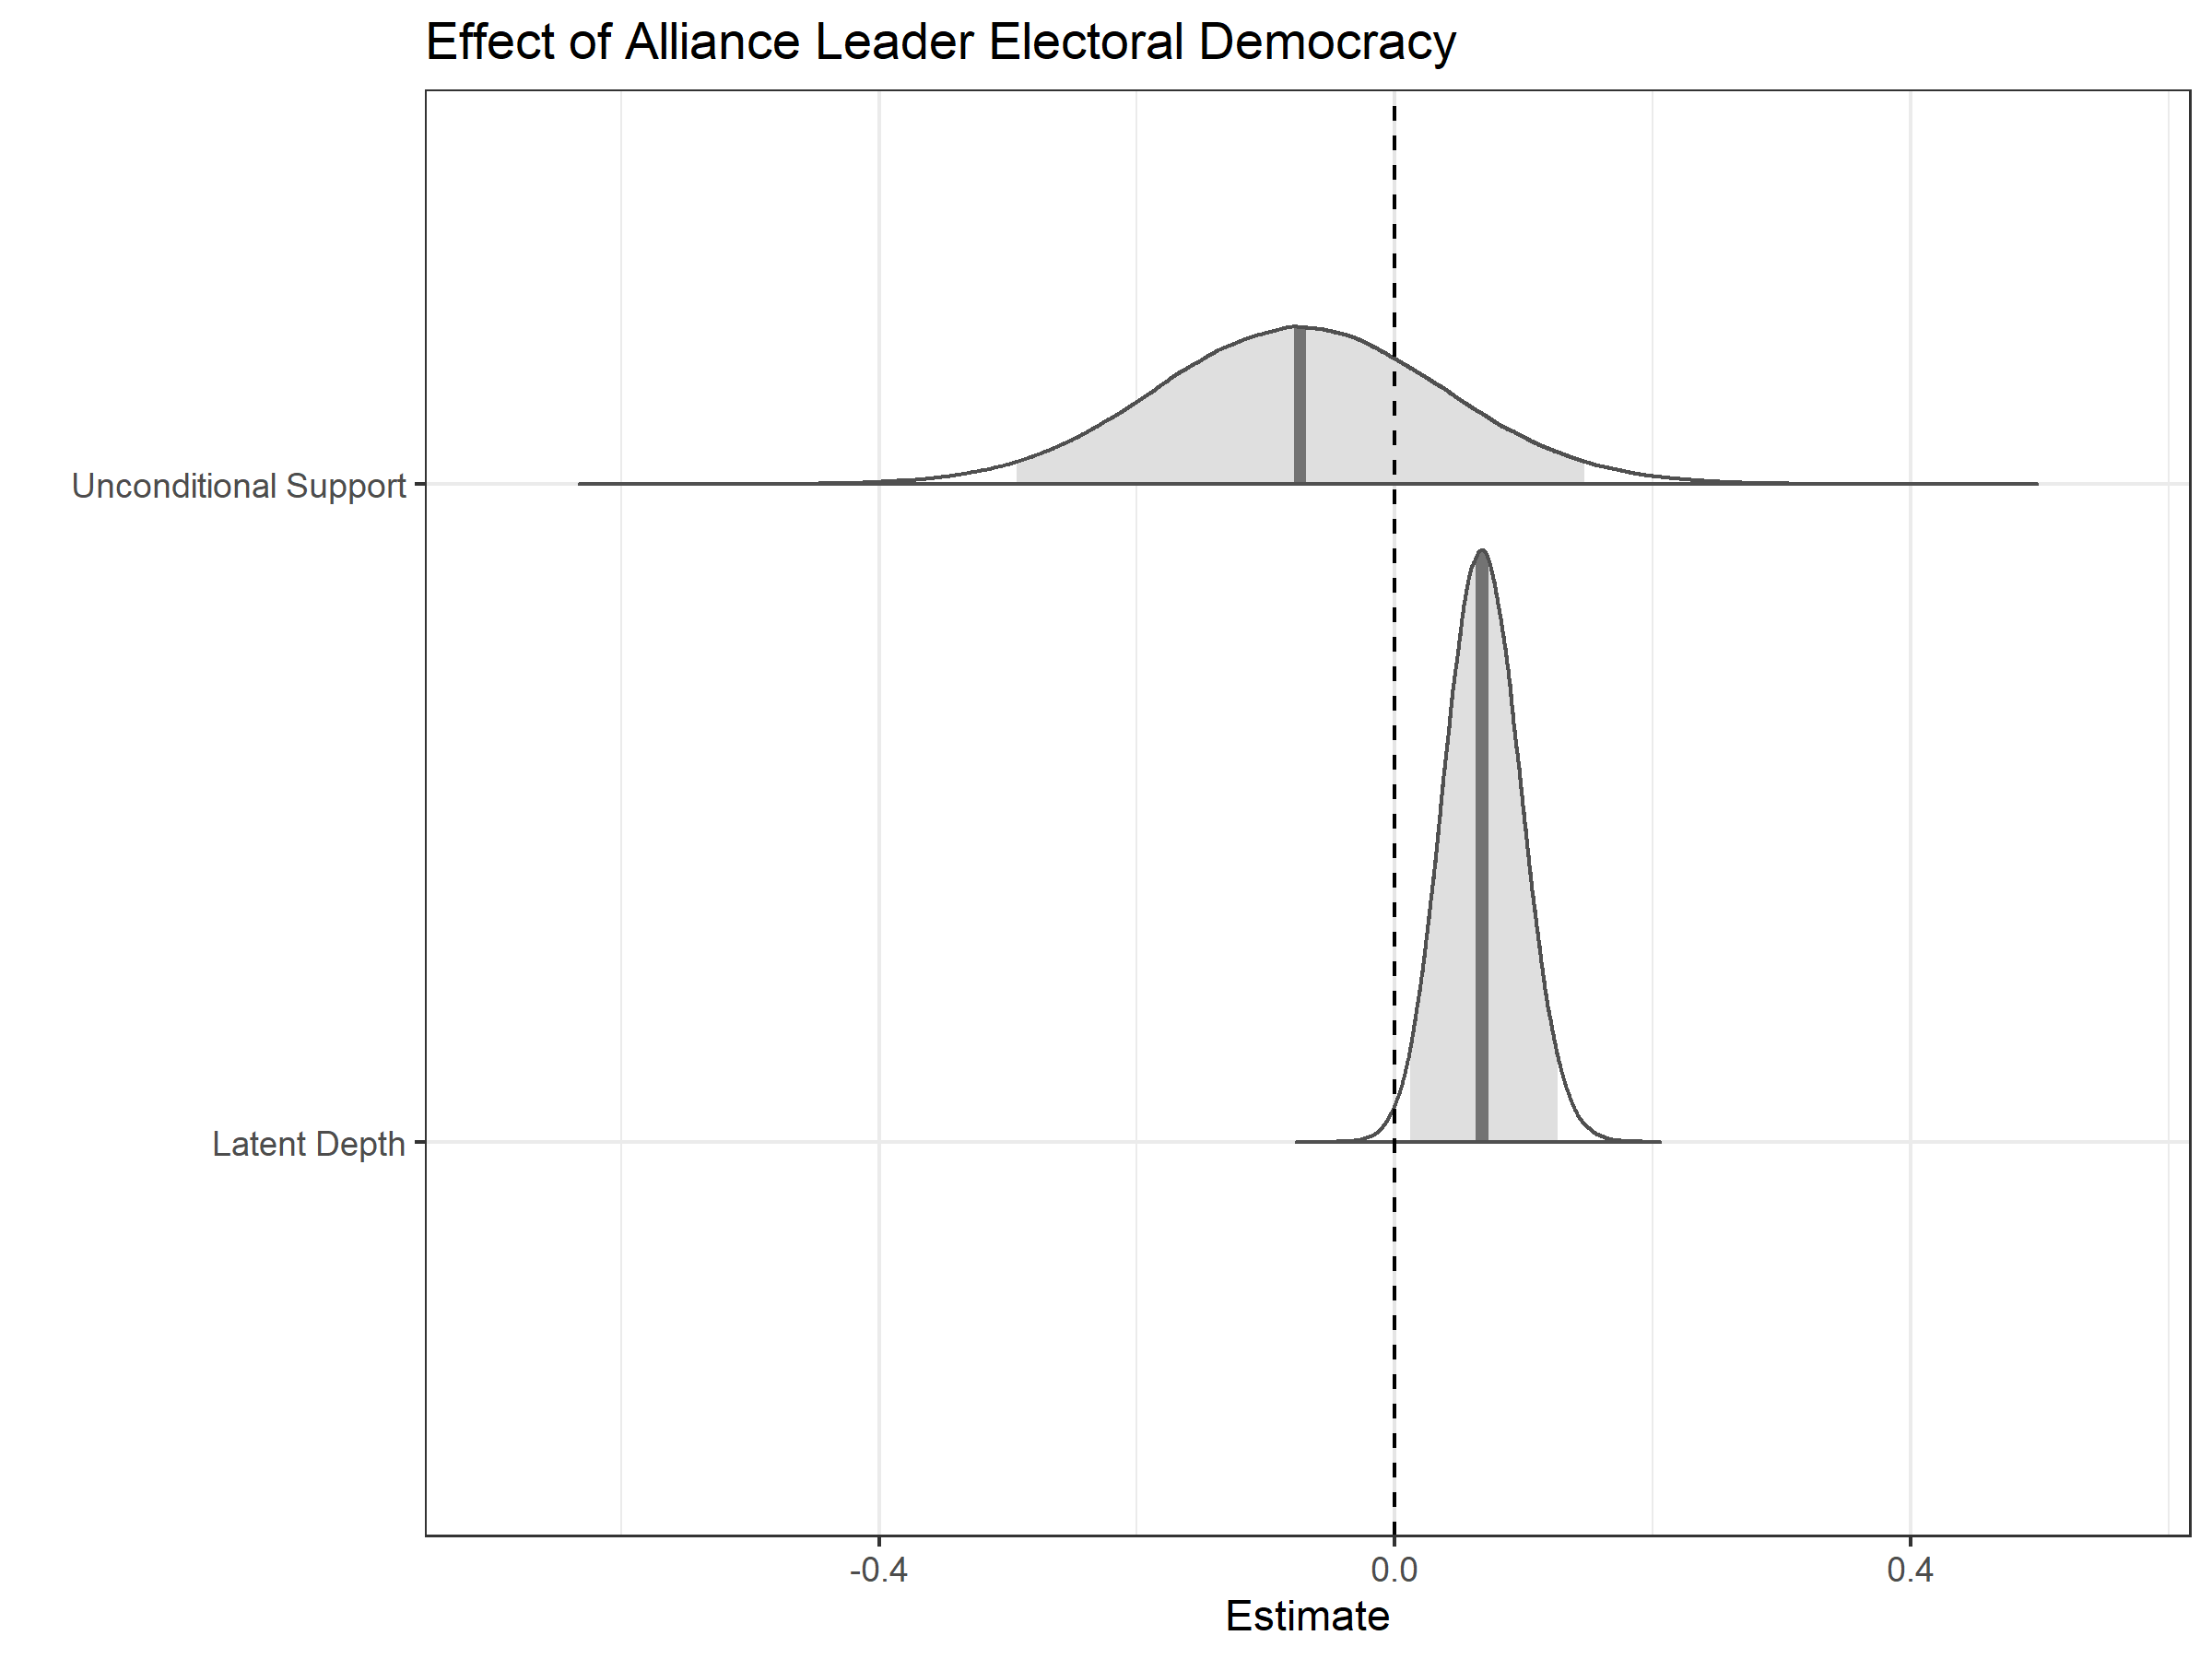
\includegraphics[width=.95\textwidth]{results-unc-depth.png}  
\caption{Estimated association between the electoral democracy and executive constraints of the most capable alliance member and treaty depth from a Bayesian model that accounts for uncertainty in the latent depth measure. The density plot shows the posterior distributions, and the shaded area summarizes the 95\% credible interval.}
\label{fig:results-unc-depth}
\end{figure}




\newpage

\singlespace
 
\bibliography{../../../MasterBibliography} 





\end{document}